\documentclass[male,czech]{kithesis}

\usepackage{graphics}
\usepackage{array}

% zde nastavte základní informace o bakalářské práci
\newcommand{\AUTOR}{Oleg Musijenko}
\newcommand{\TITULcz}{Tacit programming - návrh doménově specifického jazyka a implementace jeho interpretu} % titul v českém jazyce
\newcommand{\TITULen}{Tacit programming - design of a domain specific language and implementation of it's interpreter} % titul v anglickém jazyce
\newcommand{\KLICOVASLOVAcz}{bakalářská práce, odborný text, programování} % klíčová slova v českém jazyce
\newcommand{\KLICOVASLOVAen}{bachelor thesis} % klíčová slova v anglickém jazyce
\newcommand{\VEDOUCI}{Mgr. Jiří Fišer, Ph.D.}    

\newcommand{\PROGRAM}{Aplikovaná informatika}    
\newcommand{\OBOR}{Informační systémy}    
% nastavení fontů (liší se podle TeXovského stroje)
\iftutex
\usepackage{fontspec}
\setmainfont{Libertinus Serif} % použito je opensource písmo Libertinus, lze použít jakékoliv jiné rozumné
\setsansfont{Libertinus Sans}
\setmonofont[Scale = MatchLowercase]{Libertinus Mono}
%\setmainfont{APL385}
\newfontfamily\apl{APL385}
\usepackage{unicode-math}  
% písmo pro matematiku, vhodná písma viz  	např. https://developer.mozilla.org/en-US/docs/Mozilla/MathML_Project/Fonts
\setmathfont{Libertinus Math}
\else
\usepackage[utf8]{inputenc}
\usepackage[T1]{fontenc}
\usepackage{libertinus}

\usepackage{amsmath,amssymb}
\usepackage{libertinust1math}
\usepackage{graphicx}
\usepackage[font=small, labelfont=bf]{caption}
\fi

\usepackage[
  style=authoryear,
  backend=biber,
  citestyle=authortitle
  ]{biblatex}
\usepackage{minted}
\usepackage{listings}
\usepackage[dvipsnames]{xcolor}

% \newcommand\mkbibcolor[2]{\textcolor{#1}{\hypersetup{citecolor=#1}#2}}
% \DeclareCiteCommand{\cite}[\mkbibcolor{red}]
%   {\usebibmacro{prenote}}%
%   {\usebibmacro{citeindex}%
%    \usebibmacro{cite}}
%   {\multicitedelim}
%   {\usebibmacro{postnote}}

\definecolor{CodeBackGround}{cmyk}{0.0,0.0,0,0.05}  % light gray
\definecolor{CodeComment}{rgb}{0,0.50,0.00}         % dark green {0,0.45,0.08}

\addbibresource{bibliografie.bib}
% vylepšení vzhledu
\usepackage{microtype}
%\sloppy %odpoznámkujte pokud vám často přetékají řádky
\renewcommand{\arraystretch}{1.23} % vertikální roztažení tabulek o 23%


% Source from: https://github.com/bakerjd99/jacks/blob/master/latex/apl-lstlisting.tex
\lstdefinelanguage{apl}
{
extendedchars=true,
morekeywords={},
otherkeywords={:if,:else,:for,:in,:while,:until
,:andif,:orif,:repeat,:select,:case
,:go,:return,:try,:catch,:catchif,:catchall
,:endfor,:endwhile,:endselect,:endif,:endrepeat,:endselect},
keywordstyle=\bfseries\color{red},
sensitive=True,
morecomment=[l]{⍝}
}
\setmonofont{APL385}

\lstset{%
  basicstyle=\ttfamily\small,  
  keywordstyle=\bfseries\normalsize,  % can color key words        
  identifierstyle=,                             
  commentstyle=\slshape\color{CodeComment}, % no slanted shape in APL385    
  stringstyle=\ttfamily,                        
  showstringspaces=false,                      
  framesep=1pt,                                
  framerule=0.8pt,                              
  breaklines=true,      % break long code lines                        
  breakindent=0pt                             
}

\makeatletter
\lst@InputCatcodes
\def\lst@DefEC{%
 \lst@CCECUse \lst@ProcessLetter
  ^^80^^81^^82^^83^^84^^85^^86^^87^^88^^89^^8a^^8b^^8c^^8d^^8e^^8f%
  ^^90^^91^^92^^93^^94^^95^^96^^97^^98^^99^^9a^^9b^^9c^^9d^^9e^^9f%
  ^^a0^^a1^^a2^^a3^^a4^^a5^^a6^^a7^^a8^^a9^^aa^^ab^^ac^^ad^^ae^^af%
  ^^b0^^b1^^b2^^b3^^b4^^b5^^b6^^b7^^b8^^b9^^ba^^bb^^bc^^bd^^be^^bf%
  ^^c0^^c1^^c2^^c3^^c4^^c5^^c6^^c7^^c8^^c9^^ca^^cb^^cc^^cd^^ce^^cf%
  ^^d0^^d1^^d2^^d3^^d4^^d5^^d6^^d7^^d8^^d9^^da^^db^^dc^^dd^^de^^df%
  ^^e0^^e1^^e2^^e3^^e4^^e5^^e6^^e7^^e8^^e9^^ea^^eb^^ec^^ed^^ee^^ef%
  ^^f0^^f1^^f2^^f3^^f4^^f5^^f6^^f7^^f8^^f9^^fa^^fb^^fc^^fd^^fe^^ff%
  ^^^^20ac^^^^0153^^^^0152%
  ^^^^20a7^^^^2190^^^^2191^^^^2192^^^^2193^^^^2206^^^^2207^^^^220a%
  ^^^^2218^^^^2228^^^^2229^^^^222a^^^^2235^^^^223c^^^^2260^^^^2261%
  ^^^^2262^^^^2264^^^^2265^^^^2282^^^^2283^^^^2296^^^^22a2^^^^22a3%
  ^^^^22a4^^^^22a5^^^^22c4^^^^2308^^^^230a^^^^2336^^^^2337^^^^2339%
  ^^^^233b^^^^233d^^^^233f^^^^2340^^^^2342^^^^2347^^^^2348^^^^2349%
  ^^^^234b^^^^234e^^^^2350^^^^2352^^^^2355^^^^2357^^^^2359^^^^235d%
  ^^^^235e^^^^235f^^^^2361^^^^2362^^^^2363^^^^2364^^^^2365^^^^2368%
  ^^^^236a^^^^236b^^^^236c^^^^2371^^^^2372^^^^2373^^^^2374^^^^2375%
  ^^^^2377^^^^2378^^^^237a^^^^2395^^^^25af^^^^25ca^^^^25cb%  
  ^^00}
\lst@RestoreCatcodes
\makeatother

% \lstset{ %
%   language=Haskell,                % hlavní programovací jazyk, seznam podporovaných viz https://en.wikibooks.org/wiki/LaTeX/Source_Code_Listings
%   basicstyle=\ttfamily,    
%   showspaces=false,                % show spaces adding particular underscores
%   showstringspaces=true,           % underline spaces within strings
%   showtabs=false,                  % show tabs within strings adding particular underscores
%   frame=single,                    % adds a frame around the code
%   tabsize=3,                       % sets default tabsize to 3 spaces
%   breaklines=true,                 % sets automatic line breaking
%   breakatwhitespace=false,         % sets if automatic breaks should only happen at whitespace
%   keywordstyle=\bfseries,          % keyword style
%   commentstyle=\rmfamily,          % comment style
%   stringstyle=\itshape,            % string literal style
% }

% nastavení hypertextových odkazů a PDF metainformací
\usepackage{url} % přidává příkaz url pro sazbu url
\usepackage[unicode=true,colorlinks=true,
            citecolor=blue, linkcolor=blue,
            urlcolor=blue,
            pdftitle={\TITULcz},pdfauthor={\AUTOR},
            pdfkeywords={\KLICOVASLOVAcz}]{hyperref}
\usepackage[skip=10pt plus1pt]{parskip}
\newcommand{\haskellInline}[1]{\colorbox{gray!10}{\mintinline{haskell}{#1}}}
\newcommand{\aplInline}[1]{\colorbox{gray!10}{{\apl{#1}}}}

\pagestyle{fancy} % aktivování stylu záhlaví a zápatí z kithesis

%---------------------------------------------------------

\begin{document}
\thispagestyle{empty}
\begin{center}
{\Huge Univerzita Jana Evangelisty Purkyně \\
v~Ústí nad Labem}
\\[16pt]
{\huge Přírodovědecká fakulta}

\vspace{2cm}
\resizebox{8cm}{!}{
\includegraphics{LOGO_PRF_CZ_RGB_standard.jpg}}

\vspace{2cm}
{
\huge
\TITULcz\par

\vspace{0.5em}
\LARGE\scshape bakalářská práce
}
\end{center} 
 
\vfill
{
\large
\begin{tabular}{>{\bfseries}rl}
    Vypracoval: 	& \AUTOR\\
    Vedoucí práce: 	& \VEDOUCI\\
&\\
Studijní program:       & \PROGRAM\\
Studijní obor:          & \OBOR\\
\end{tabular} 
}
\vspace{1.5cm}
\begin{center}
\Large\scshape   Ústí nad Labem \the\year
\end{center}

\cleardoublepage
\thispagestyle{empty}

\textbf{\textsf{Cíl bakalářské práce}}

Cílem bakalářské práce je ukázat výhody a nevýhody tacit přístupu k programování. Výstupem práce bude návrh vlastního doménově specifického jazyka (DSL), který
bude využívat tacit programming, a navazující pilotní implementace jeho interpretu.
Návrh jazyka by se měl soustředit na následující body:\\
• přehledná syntaxe,\\
• možnosti použití vysokoúrovňových nástrojů pro překlad a podporu běhu programu (např. LLVM v Haskellu) včetně parsování jazyka (např. Parsec v Haskellu),\\
• efektivita při vykonávaní,\\
• případná podpora paralelních výpočtů

\cleardoublepage
\thispagestyle{empty}

\textbf{Prohlášení}

Prohlašuji, že jsem tuto bakalářskou práci vypracoval\ifthenelse{\boolean{feminum}}{a}{} samostatně a použil\ifthenelse{\boolean{feminum}}{a}{}
jen pramenů, které cituji a uvádím v přiloženém seznamu literatury.

\vspace{1em}
Byl\ifthenelse{\boolean{feminum}}{a}{} jsem seznámen\ifthenelse{\boolean{feminum}}{a}{} s tím, že se na moji práci vztahují práva a povinnosti vyplývající ze zákona č. 121/2000 Sb., ve znění zákona č. 81/2005 Sb., autorský zákon, zejména se skutečností, že Univerzita Jana Evangelisty Purkyně v Ústí nad Labem má právo na uzavření licenční smlouvy o užití této práce jako školního díla podle § 60 odst. 1 autorského zákona,s tím, že pokud dojde k užití této práce mnou nebo bude poskytnuta licence o užití jinému
subjektu, je Univerzita Jana Evangelisty Purkyně v Ústí nad Labem oprávněna ode mne požadovat přiměřený příspěvek na úhradu nákladů, které na vytvoření díla vynaložila, a to podle okolností až do jejich skutečné výše.

\vspace{1em}
V Ústí nad Labem dne \today \hspace{0.3\textwidth} Podpis:


\clearpage
\thispagestyle{empty}
~\vfill

\begin{flushright}
  Děkuji vedoucímu práce Mgr. Jiřímu Fišerovi, Ph.D.\\ za neocenitelné rady a pomoc při tvorbě bakalářské práce.

  Též chci poděkovat své ženě, Anetě Musijenko, \\ za neustálou podporu během psaní práce.
\end{flushright}

\cleardoublepage
\thispagestyle{empty}

\textbf{\textsf{Abstrakt}}

\textsc{\TITULcz}

% Abstrakt shrnuje základní motivaci práce (kontext), hlavní cíl a následně jednotlivé
% autorské kroky k~jeho splnění (co bylo uděláno od úvodních rešerší, přes návrh, implementaci k případnému nasazení. Minimální rozsah je 800 znaků (maximální půl strany).

\textbf{\textsf{Klíčová slova}}

% seznam klíčových slov (obecných termínů vystihujících téma práce) v počtu dva až deset 

\vspace{1em}
\hrulefill
\vspace{1em}

\textbf{\textsf{Abstract}}

\textsc{\TITULen}

Translation of Czech abstract.

\textbf{\textsf{Key words}}

Translation of czech key words.

{
  \hypersetup{linkcolor=black}
  \tableofcontents
}

\addchap{Úvod}

Programovací paradigma je způsob myšlení a přístupu k návrhu, 
strukturování a implementaci počítačových programů. 
Definuje sadu pravidel, postupů, technik a konceptů, které určují způsob,
jakým se programy píší a organizují. Paradigma poskytuje rámec pro definici a 
řešení problémů v programování.

Některé z nejznámějších programovacích paradigmat zahrnují:

\section{Procedurální paradigma}
Zaměřuje se na sekvenci instrukcí, 
které jsou vykonávány postupně. 
Program je rozdělen na procedury a funkce, které provádějí určité operace. Příkladem takového 
paradigmatu je jazyk C, GOlang a Assembly. Zde se programátoři často setkávají s nutností
manuální správou paměti (\textit{malloc}, \textit{free}).

\section{Objektově orientované paradigma - OOP}
Klade důraz na objekty a jejich interakce. 
Program je strukturován kolem tříd, které obsahují data (atributy) a metody (funkce), 
které s těmito daty pracují. Toto paradigma je obohaceno o \textbf{polymorfismus}.
Vývojáři si mohou OOP představit jako nadmonžinu Procedurálního paradigmatu.

V závislosti na programovacím jazyce, 
vývojáři mohou vužívat automatickou správu paměti díky \textit{garbage collectoru}, kde 
tuto správu paměti vužívají C\# a Java. Pokud je zapotřebí manuální správa paměti, je zde
C\+\+ nebo Rust. Rust je zajímavý tím, že využívá \textit{borrow checker} a má napodobit
chování smart pointerů.


\section{Funkcionální paradigma - FP}
Jedná se o deklarativní způsob programování, kde funkce jsou 
považovány za základní stavební bloky programu. 
Funkcionální jazyky mají za cíl minimalizovat mutaci dat a preferovat neměnné \textit{immutable}
struktury. 
To přispívá ke stabilitě, zjednodušené paralelizaci a eliminaci některých typů chyb. 
Jazyky jako Lisp a jeho dialekty, oCaml, Closure, F\# a Haskell 
jsou běžnými příklady funkcioního programování.

V jednotlivých funkcionálních jazycích je povolena různá míra mutace dat. 
Například jazyk F\# umožňuje mutaci dat kdekoli v programu, což je částečně záměrem, 
aby oslovil uživatele jazyka C\#. Na druhou stranu, 
v jazyce Haskell jsou mutace omezeny v IO monádě a data musí být uloženy 
ve specifických typech jako IORef, STRef nebo MVar. Takto Haskell 
pomáhá udržet jasnou separaci mezi čistým funkcionalním kódem a kódem, 
který se zabývá měnícím se stavem nebo interakcí s okolím.


Je důležité si uvědomit, že míra povolené mutace dat se může lišit mezi jednotlivými funkcionálními jazyky a je závislá na jejich návrhu a filozofii. Každý jazyk si volí kompromis mezi funkcionalitou a striktností v oblasti mutace, aby splňoval požadavky svých uživatelů a cílů, které si klade.

\section{Cíl práce}

Cílem práce je vytvoření doménově specifický konkuretní jazyk, který usnadní přehled business logiky a zlepší 
vývojářské prostředí (developer experience) se zaměřením na \textit{tacit} - "beztečkové" paradigma.
V práci budou ukázky, jak
tacit programming vypadá a budou vyzdvyženy argumenty proč s tacit programmingem
vůbec pracovat.
Do tohoto paradigmatu spadají jazyky APL rodiny. 
Ukázky v této práci potvrdí, že jazyky které nebyly primárně navržené jako "beztečkové" 
umožňují v tomto stylu psát.

Tato bakalářská práce předpokládá, že čtenář zná základy funkcionálních jazyků a obzvlášť Haskellu, 
protože návrh je vytvořen v Haskellu pomocí knihoven jako je Parsec a MTL (Monad Transformer).

\chapter{Tacit programming}
\textbf{Tacit programming} je programovací styl, 
který klade důraz na skládání a řetězení funkcí a není založen na explicitní specifikaci parametrů funkcí.
Pro základní ukázky bude využit JavaScript jelikož se jedná o jeden z nejpopulárnějších jazyků. 
Základní principy funkcionálního a tacit programování jsou v jazyce JavaScript,
jelikož se jedná o jeden z nejvíce populárních programovacích jazyků a v základu má již funkcionální možnosti.
Detailnější principy jsou psány v Haskellu.
\begin{minted}{js}
  fetch("APIURL")
  .then(x => fancyFunction(x))
  .then(x => console.log(x))
  .catch(e => console.error(e))
\end{minted}

Zde se řetězí funkce zpětného volání ("Callbacks").

Tento postup je běžný u JavasSript programátorů, ale bohužel má jednu malou nevýhodu.
Tvoří se zde zbytečná anonymní funkce ("arrow function nebo-li šipková") a pokud bychom prohlubovali čím dál víc 
zásobník volání, mohou nám tyto anonymní funkce zabírat paměť a během debuggingu nám tento styl zápisu "znečišťuje" 
zásobník volání. 

\begin{minted}{js}
  fetch("APIURL")
  .then(fancyFunction)
  .then(console.log)
  .catch(console.error)
\end{minted}

Přepsaná ukázka je logicky ekvivalentní k té předešlé. Zásadní rozdíl je ten, že se nemusí na paměťový zásobník ukládat kontext anonymní funkce 
a explicitně se nepředávají parametry funkce. Tudíž se jedná o \textit{tacit} zápis.

Následující úryvek ukazuje, jak funguje \textbf{currying} a proč souvisí s tacit programováním.
\begin{minted}{js}
const curry = (f) => a => b => f(a,b);
const sayHello = (a, b) = `Hello ${a} from ${b}`;
const applyToFunctionArray = 
    (input,...args) => args.map(a => a(input))
const partiallyAppliedData = ["A", "B", "C"].map(curry(sayHello)); 
// [(b) => "Hello A from ${b}", 
//  (b) => "Hello B from ${b}", 
//  (b) => "Hello C from ${b}"]
const partiallyAppliedData2 = ["A", "B", "C"]
                              .map(curry(sayHello)(1)); 
// ["Hello A from 1", 
//  "Hello B from 1", 
//  "Hello C from 1"]
\end{minted}
Curry funkce transfomuje existujícé funkci tak, že máme pro každý argument vlastní vracející funkci. 
Z funkce \textbf{f(a,b,c,d)} vzniká funkce \textbf{f(a)(b)(c)(d)} (\cite{Currying}).
V čem je toto výhodné?
Například je zde uvedené pole, které se skládá z částečně aplikovaných funkcí. 
Takto může programátor naiterovat odpověď ze serveru do objektu z předchozí ukázky,
které je závislé na třeba na uživatelském vstupu. 

Zajímavější část je u \textit{partiallyAppliedData2}. Curryovaná funkce vrací 
funkci, jež očekává vstupní parametr, aby byla vyhodnocena. Tento princip je důležitý
pro lenivé vyhodnocení, který využívá Haskell.

Může zde padnout argument, že v našem případě se curryování nachází pouze pro funkci,
která prijímá dva argumenty. Zde je definice funkce, která převádí jakoukoliv funkci na curryovanou.

\begin{minted}{js}
const curry = (f) => (..args) => args.length >= f.length ? 
  f.apply(this, args) : (...args2) => 
    curry.apply(this, args.concat(args2));
\end{minted}
\section{Principy a odlišnosti od klasického paradigmatu}

Procedurální paradigma se zaměřuje na psaní procedurálních instrukcí.
Typickým příkladem tohoto paradigmatu je programovací jazyk C, protože se
jedná o standard, tak v následujících příkladech budu porovnávat jazyk C s jazykem Haskell.
Haskell je primárně funkcionální jazyk, tento jazyk umožňujě psát funkce
v "beztečkovém" stylu. 

Následující příklad sumace:

\textbf{Haskell}
\begin{minted}{Haskell}
sumCustom:: (Traversable t, Num a) => t a -> a
sumCustom = foldr (+) 0
\end{minted}
\pagebreak
\textbf{C}
\begin{minted}{c}
int sum(int* arr, size_t numOfElements)
{
    int acc = 0;
    
    for(int i = 0; i < numOfElements; i++)
    {
        acc += *(arr + i);
    }
    
    return acc;
}
\end{minted}
Na příkladu jde vidět, že beztečkový styl zápisu je opravdu kompaktní. 
V Haskellu není třeba zasahovat do parametrů funkcí.
Tento příklad je založen na podstatě tacit programmingu.
Co se týče algoritmizace, tacit programming je známý pro vytváření 
algoritmických řešení pomocí pouze jednoho řádku kódu. 

Na dalším příkladě si ukážeme fibonnacciho posloupnost.
\textbf{Haskell}
\begin{minted}{Haskell}
-- Haskell je lenivý jazyk a proto je možné vytvořit nekonečnou 
-- fibonnacciho posloupnost a z té si vzít jen potřebný počet čísel 
fibonacci:: Num a => Int -> [a]
fibonacci = (flip take) fibonacciInfinite
  where
    fibonacciInfinite:: Num a => [a]
    fibonacciInfinite = scanl (+) 0 (1:fibonacciInfinite)
\end{minted}

\vfill
\pagebreak

\textbf{C}
\begin{minted}{c}
void fibonacci(int* arr, size_t numOfElements)
{
    if(numOfElements > 0)
    {
      arr[0] = 0;
    }
    if(numOfElements > 1)
    {
      arr[1] = 1;
    }
    for(int i = 2; i < numOfElements; i++)
    {
      arr[i] = arr[i - 1] + arr[i - 2];
    }
}
\end{minted}

Z pohledu imperativního programátora implementace v C je zcela jasná. Funkce přijímá ukazatel na
pole a modifikuje toto pole. Zatímco v Haskellu tato implementace může být matoucí. Funkce scanl je 
velice podobná funkci foldl, jen místo vracení akumulátoru, tak vrací průběžně vypočtené hodnoty.

\section{Debugging}

Debugging je zásadní činností při vývoji softwaru, která umožňuje identifikovat, 
analyzovat a odstraňovat chyby ve zdrojovém kódu. 
Proces debuggování je obzvláště důležitý v imperativních a objektově orientovaných jazycích, 
které často disponují vyspělými debugovacími nástroji. 
V těchto jazycích je očekáváno sekvenční vykonávání instrukcí, 
což usnadňuje postupné sledování jejich provádění. 
Inspekce zásobníku volání představuje 
další přirozenou součást debuggingu v těchto jazycích.

V případě lenivého jazyka Haskell však debugging přináší značné obtíže. 
Haskell využívá mechanismu lenivého vyhodnocování, což znamená, 
že hodnoty jsou vypočteny až ve chvíli, kdy jsou skutečně potřeba. 
Tato vlastnost komplikuje proces sledování výpočtu a identifikaci chyb. 
I přes existenci několika debuggovacích nástrojů pro Haskell může 
debugging pro zkušeného vývojáře představovat opravdovou výzvu. 
Zmatek může vznikat zejména při určování, 
kde a jak byla konkrétní proměnná získána, 
neboť její hodnota je vypočítána až v okamžiku, 
kdy je použita.
\pagebreak

Naštěstí Haskell nabízí možnost využití REPL 
(Read - Eval - Print - Loop) prostředí, 
které umožňuje interaktivní evaluaci výrazů a postupné zkoumání jejich chování. 
REPL tak může sloužit jako užitečný nástroj pro rychlé testování 
a experimentování s funkcemi a výrazy. 
Přítomnost REPL v Haskellu zčásti kompenzuje obtíže spojené 
s debuggingem a poskytuje prostředí pro analýzu a ladění kódu.

\section{Rešerše existujících implementací - APL}

Jazyk APL je jazyk orientovaný na pole nebo-li \textit{array oriented programming language} se 
syntaxí zaměřenou na tacit programming. V APL jsou všechny data reprezentovány jako pole 
a všechny pole jsou skládány ze skalárů a nad 
nimi jsou dělané matematické operace s poněkud netradiční syntaxí. Totiž každá 
předem jazykem definovaná funkce je přidělená ke speciálnímu UTF-8 chararakteru. 
Například funkce pro přirozený logaritmus je {\apl '⍟'} nebo zaokrouhlení nahoru či dolů 
jsou {\apl '⌈' '⌊'}.
Každá funkce se dá zapsat monadicky či dyadicky. 

Monadický zápis má argument operandu na pravé straně:
\aplInline{-5    ⍝ monadic}

Dyadický zápis má argumenty na obou stranách operandu:
\aplInline{10-7  ⍝ dyadic}

Jelikož všechny pole jsou tvořeny skaláry, tak operace "ignorují" strukturu pole a pracují přímo 
s obsahem pole.

\begin{lstlisting}[language=apl,extendedchars=true]
  ⍳6          ⍝ 6 integers starting from the origin.
0 1 2 3 4 5
  1+⍳6        ⍝ Add 1 to the 6 integers starting from the origin.
1 2 3 4 5 6
  2×⍳6        ⍝ Multiply by 2 the 6 integers starting from the origin.
0 2 4 6 8 10
\end{lstlisting} 
(\cite{WhyAPLIsWorthKnowing})

Pokud pole jsou u dyadického zápisu stejné délky, tak jsou hodnoty vypočteny jako jednotlivé 
skaláry.

\begin{lstlisting}[language=apl,extendedchars=true]
  100 0 1 × 2 3 4
200 0 4
\end{lstlisting}

Operátory jsou vyhodnocovány z prava do leva.

\begin{lstlisting}[language=apl,extendedchars=true]
  24 ÷ 12 6 - 4 2   ⍝ -> 24 ÷ 8 3
3 6
\end{lstlisting}

Booleany jsou reprezentovány jako 1 (True) a 0 (False). Zde je ukázka algoritmu, kde 
se sečte sekvence přirozených čísel (včetně nuly, ale při součtu nemá vliv), 
která jsou dělitelná buď třemi nebo pěti.

\begin{lstlisting}[language=apl,extendedchars=true]
  Euler1 ← {+/((0=3|⍵)∨(0=5|⍵))/⍵}

  Euler1 ⍳1000
234168
\end{lstlisting}

Funkce \aplInline{(0=3|⍵)∨(0=5|⍵) ⍝ '|' - modulo, '=' is equal operator} zjišťuje zda-li je číslo
dělitelné třemi nebo pěti a vrací 0 nebo 1. Operátor \aplInline{/} funguje jako replicate 
(pokud je spojené s dalším operátorem, tak funguje jako reduce). 
Jelikož je vyhodnocování z prava do leva, tak pokud argument funkce je 
například 7 a 12 tak: 

\aplInline{((0=3| 7 12)∨(0=10 | 7 12))/7 12 ⍝ Result: 12}.

Toto celé funguje jako filtrování, 
kombinací operátorů \aplInline{+/} se udělá suma výsledků.

Lze si ale povšimnout, 
že výše zmíněný příklad není zapsán v tacit stylu jelikož využívá argument \aplInline{⍵}.
Je možné napsat zmíněný příklad do tacit stylu, ale zároveň se zvyšuje komplexita porozumění.
\begin{lstlisting}[language=apl,extendedchars=true]
  Euler1 ← +/((0=3|⊢)∨(0=5|⊢))×⊢
\end{lstlisting}

(\cite{CzechApl})

\section{Kdy využít tacit zápis}

Tacit styl může být mocný a elegantní.
Zde je několik argumentů, proč by se měl tacit zápis využít:

\textbf{Kompaktnost a elegance:}
Tacitní zápis může často zredukovat kód na mnohem kratší a elegantnější formu, 
což může zvýšit čitelnost a snížit objem psaného kódu.

\textbf{Snížení chybovosti:}
Vzhledem k tomu, že tacitní zápis minimalizuje použití proměnných a stavu, 
může to snížit možnosti chyb spojených s nechtěnými efekty a nekonzistencemi v datech.

\textbf{Výkonové optimalizace:}
V některých případech může tacitní zápis vést k efektivnějšímu kódu, 
protože se snižuje zbytečná manipulace s proměnnými a daty.

\textbf{Snížení náročnosti na paměť:}
Tacitní zápis může minimalizovat požadavky na paměť tím, 
že eliminuje nutnost uchovávat mezivýsledky v proměnných.

\textbf{Zvyšuje jasnost:}
V některých případech může tacitní zápis zvýšit jasnost kódu tím, 
že se soustředí na to, co se děje (funkce a operace), 
a minimalizuje odvádějící pozornost od proměnných a argumentů.

\textbf{Kód s méně chybami:}
S minimálním množstvím stavových proměnných a 
nečekaných efektů může být kód napsaný v tacitním stylu méně náchylný k chybám.

\textbf{Přenositelnost:}
Tacitní zápis může být často snadněji přenositelný mezi různými jazyky nebo platformami, 
protože se soustředí na základní funkce a operace.

%%%%%%%%%%%%%%%%%%%%%%%%%%%%%%%%%%%%%%%%%

\section{Kdy se vyhnout tacit zápisu}

Bohužel tacit styl také může být obtížný pro programátory, 
zejména pokud nejsou na tento způsob programování zvyklí. 
Zde jsou argumenty proti tacit stylu:

\textbf{Složitost čtení a porozumění:} 
Tacitní styl může být velmi těžko čitelný a obtížný k pochopení, 
což může způsobit problémy v týmu a při údržbě kódu. 
Programátoři by měli být schopni snadno rozumět kódu,
který píšou, a kód napsaný v tacitním stylu může být matoucí.

\textbf{Náročná údržba:}
I když může být výrazně kratší, 
kód napsaný v tacitním stylu může být obtížný k úpravám a opravám chyb. 
Programátoři, kteří nejsou zvyklí na tento styl, 
budou mít problémy s debugováním a vylepšováním kódu.

\textbf{Nepodporované vývojářské prostředí:}
Některé programovací jazyky a prostředí nejsou vhodné pro zápis ve formě tacit, 
což může být dalším důvodem, proč by nemělo být programátorům vnucováno.

\textbf{Ztráta flexibility:}
Tacitní styl může omezit flexibilitu programátorů při psaní kódu.
Může být obtížnější provádět změny a úpravy v kódu, což může zpomalit vývoj.

\textbf{Vzdělávací nároky:}
Programátoři, kteří nejsou obeznámeni s tacitním stylem, 
budou muset investovat čas a úsilí do jeho pochopení a osvojení. 
To může zpomalit vývojový cyklus a zvyšovat náklady na vývoj.

\textbf{Nedostatek standardů:}
V různých programovacích jazycích mohou být různé konvence a 
standardy pro zápis ve formě tacit. To může způsobit nekonzistenci a zmatek mezi programátory.

\textbf{Kompromisy na úkor čitelnosti:}
Někdy se programátoři mohou pokoušet dosáhnout krátkého kódu na úkor čitelnosti a jasnosti. 
To může vést k nepřehledným a těžko udržovatelným programům.

%%%%%%%%%%%%%%%%%%%%%%%%%%%%%%%%%%%%%
\chapter{DSL - principy a využití}
DSL (Domain Specific Language) jsou jazyky, které se zaměřují na specifickou doménu problematiky.
Obecně DSL jazyky jsou mnohem jednodušší než jejich plnohodnotné protějšky. Výhodou je, že 
náročnost učení je mnohem nižší než u GPL (General Purpose Language). Zároveň při potřebě 
expertů na specializovaný obor, nepotřebují znát detaily 
implementace algoritmů, ale místo toho pokud budou mít přístup rovnou k DSL - výpočet šikmosti stěny budovy,
hodnota cukrů v krvi pacienta, tak mohou plnit svojí práci o mnohem efektivněji. (\cite{DomainSpecificLanguages})

\section{Web a enterprise}
Jedním z nejrozšířenejších DSL jazyků je ze světa webu a to \textbf{HTML a CSS}. HTML se zaměřuje na vytvoření rámce pro zobrazení textu,
zatímco CSS se zaměřuje na stylizaci webu pomocí DOM selectorů. Pravdou je, že pro CSS se nenachází žádný 
protocol a proto v různých webových enginech, můžete dostat různé výsledky. Příkladem z praxe je zpracování
fontů.

Též existují jazyky DSL, které jsou specifické pouze pro jednu dannou enterprise aplikaci, kde její implementace
často spočívá na bázi XML nebo podobného formátu jako je např YAML. Zde DSL slouží například pro 
zjednodušení UI nebo business logiky. Třeba pro porovnání \textbf{XAML} pro .NET platformu zjednodušuje logiku, 
stylizuje UI a zároveň zbavuje potřeby tvoření "glue" kódu, který je vygenerován automaticky.

\section{Grafické DSL}
DSL se též týká programů co běží na grafických kartách. 
Renderovací programy jsou též známé pod pojmem \textit{shader}.
Každá grafická knihovna má vlastí DSL jazyk, který jsou velmi
podobné jazyku C. Všechny renderovací jazyky prochází takzvanou 
\textit{graphic pipeline}. OpenGL a Vulkan využívají pro rendering 
OpengGL Shading Language (GLSL). OpenGL kompiluje GLSL během runtime 
programu zatímco Vulkan využívá předkompilovaného GLSL bytecode nazývaný SPIRV.

Grafické karty se nevyužívají pouze pro rendering jelikož mají širokou škálu
využitelnosti. 
Třeba \textit{CUDA} vyvinutý firmou NVIDIA 
využívá dnešní architekturu grafických karet pro paralelní výpočet 
velkoobjemných dat, kde tuto techniku využívají dnešní algoritmy pro 
strojové učení. 

\section{Ostatní DSL}
Další jazyk který je velice využíván v hardwarovém prostředí je \textbf{VHDL} nebo \textbf{Verilog}. Tyto DSL jsou zaměřená
na simulaci obvodů pomocí FPGA (hradlových polí). 
Pro kompilaci projektů existuje \textbf{makefile} a je nejčastěji spárován s C/C++. 
Jsou zde DSL pro "continuous integration and deployment". 
Různé firmy co nabízejí online repositáře se v tomto budou trochu lišit, ale
většina z nich poskytují jakousi formu automatizace vydání programu do oběhu. Toto poskytují firmy jako je GitHub,
GitLab nebo Azure Dev Ops. Na GitHubu pomocí YAMLu se dají sepsat konfigurační soubory 
na testování a deployment.

{\centering
\captionof{figure}{Výstřižek z GitHub Actions}
\resizebox{16.9cm}{!}{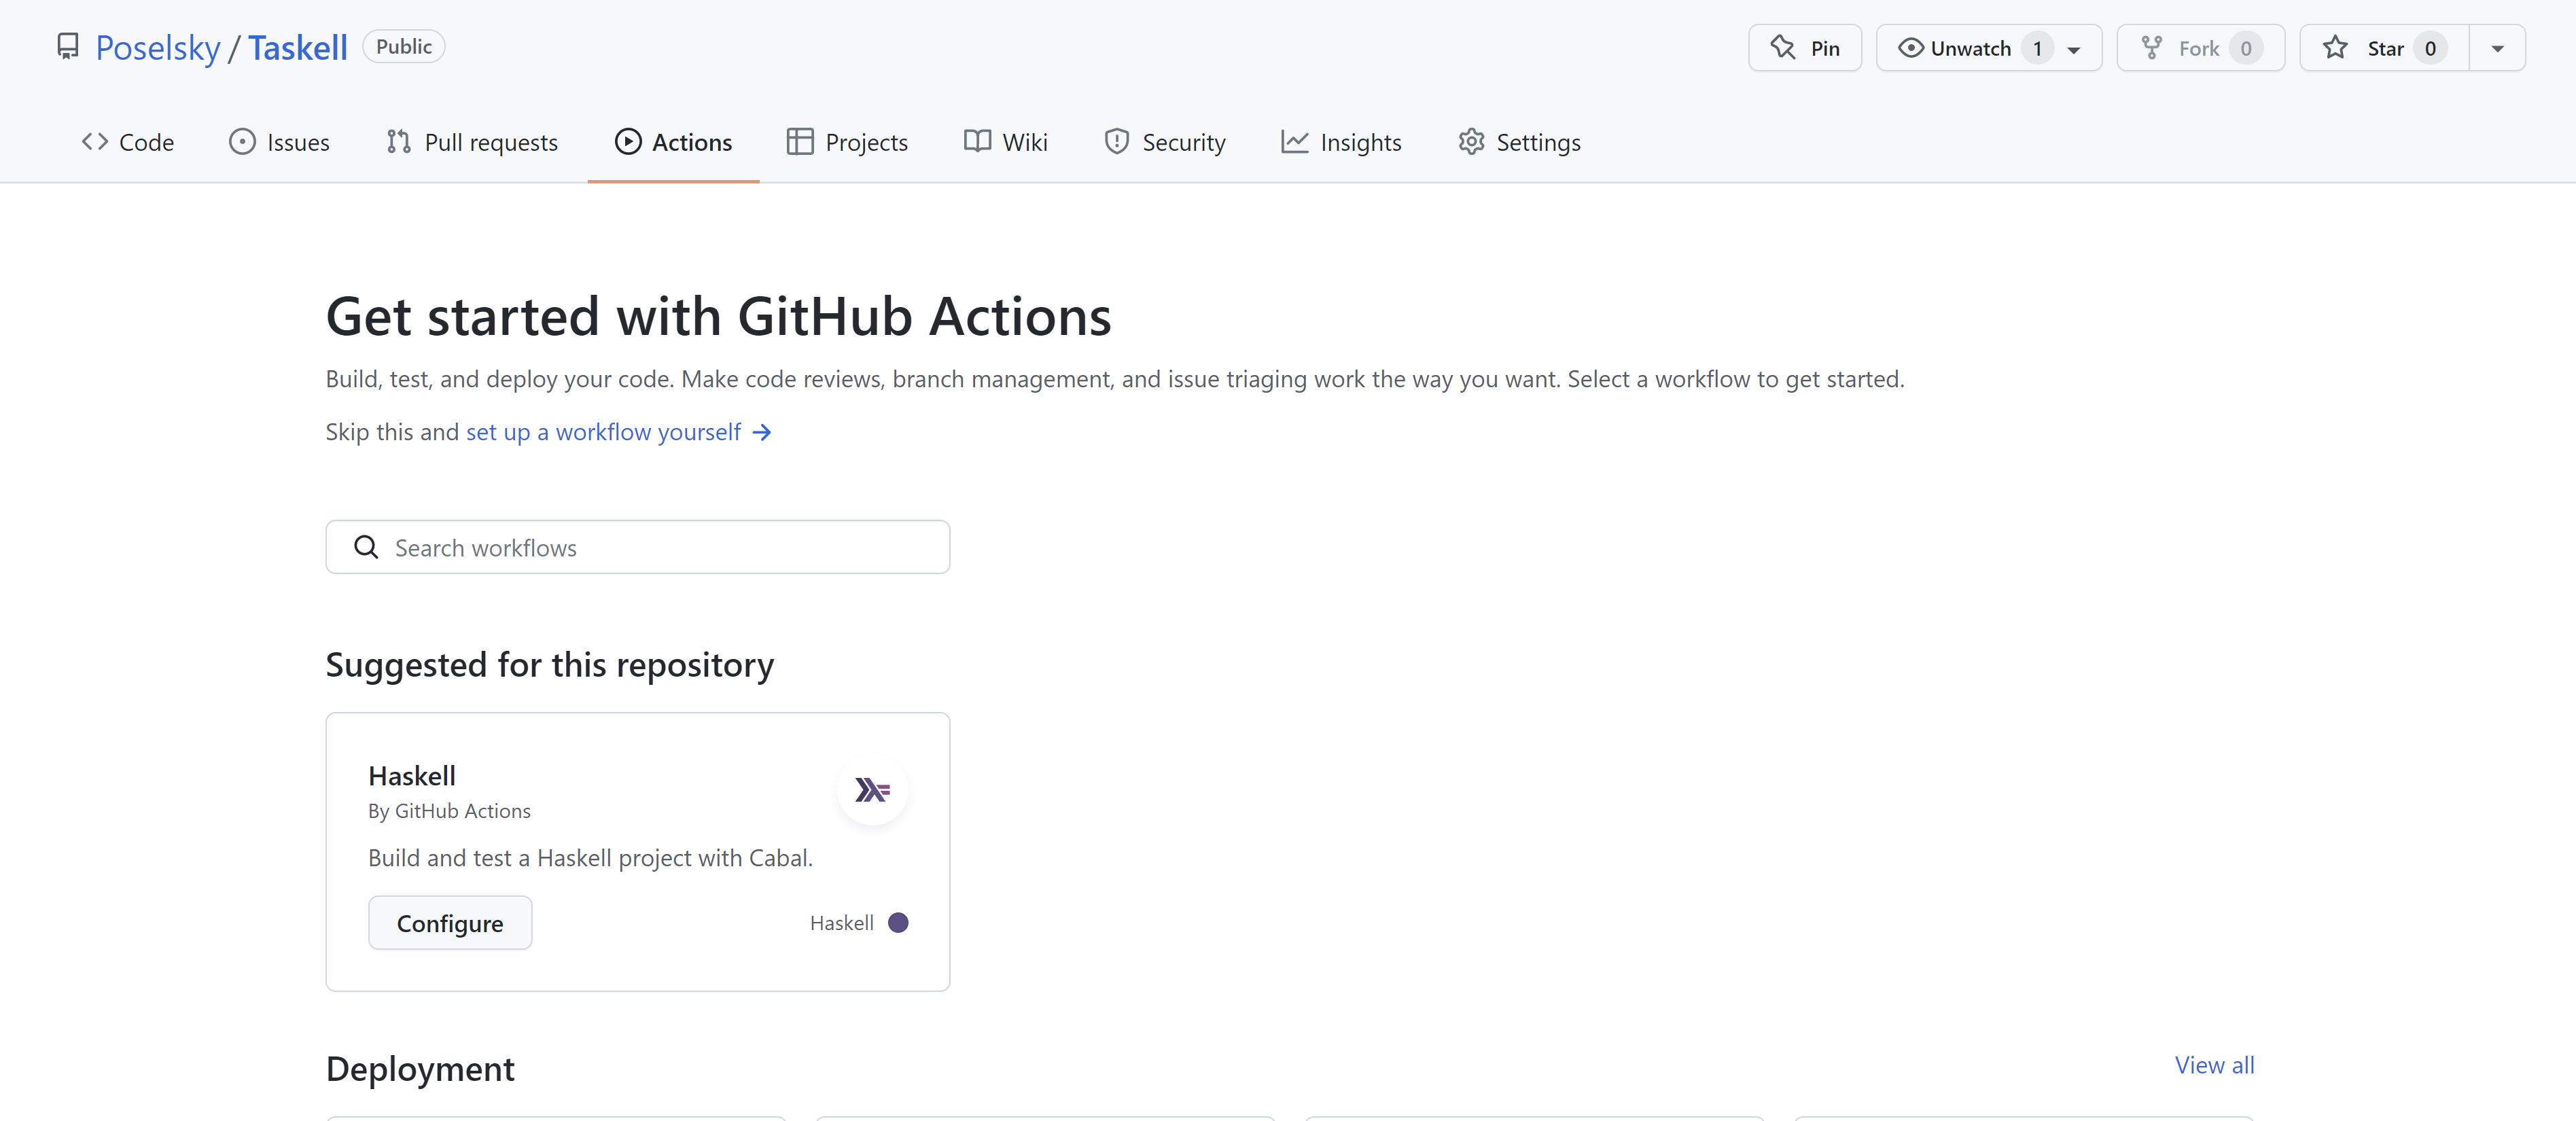
\includegraphics{Deployment.PNG}}
}

\chapter{Návrh vlastního DSL}
Pro návrh DSL je hlavní vědět o jakou doménu problematiky se jedná.
Zatím neexistuje žádná DSL implementace pro konkurenci či paralelizaci vysokého objemu dat.
Příkladem vysokého počtu dat je vzorek signálu a 
detailnější zpracování takového vzorku je časově velice náročné. Tato časová náročnost může být vyřešena právě zmíněnou
konkurencí, či paralelizací problému. 
Toto DSL je pojmenované jako \textbf{Haskelyzer}.
Pro řešení této problematiky byl zvolen Haskell, jelikož se zdá jako nejoptimálnější.
Pro rozbor jazyka byly komunitami vytvořené knihovny (Parsec, MegaParse, AttoParsec),
obsahuje mechaniky tacit programmingu, 
je staticky silně typovaný a díky monádám, řešení okrajových případů je donucené GHC kompilátorem.

\setlength{\parindent}{0pt}
Návrh danného jazyka:

\begin{minted}{haskell}
[CompileTime]
{
  let exampleCSV = "example.csv" :
    (a,Int)
    (b,Float)
    (c,String)
}

let concurrentProcess = exampleCSV | kalmanFilter 
                                   | gaussianFilter 
                                      

let nestedConcurrentProcess = exampleCSV | kalmanFilter | sum
                                                        | product
                                         | gaussianFilter

let guiMainLoop = mainLoop | calculateMainState -> writeToEventQueue
                           | gatherEventQueue -> fireEvents
\end{minted}

\section{Vysvětlení gramatiky jazyka}

Celý proces je závislý na \textit{Template Haskell} mechanismu. Díky tomuto mechanismu jsou k dispozici části kompilátoru, které umožní generovat kód dle specifikace.

Vytvoří se funkce \textit{exampleCSV}, která vrací obsah csv souboru. Při procesu kompilace se provádí kontrola, zda v csv souboru existuje dvojice "(a, Int)", kde "a" představuje název sloupce a všechny hodnoty ve sloupci "a" jsou typu "Int".
Díky atributu \textit{CompileTime} je možné vytvořit funkci \textit{exampleCSV} bez nutnosti použití IO monády. Jednou z nevýhod této metody je, že při spuštění programu se zaplní paměť, protože obsah csv souboru je součástí samotného spustitelného programu.
Nicméně díky tomu není nutné používat IO monádu a obsah csv souboru je k dispozici kdekoliv v programu.

Funkce \textit{concurrentProcess} vytvoří funkci typu \haskellInline{IO ([a],[b])} a předpokládá, že v programu jsou definované a implementované funkce
\haskellInline{kalmanFilter:: CSV -> [a]} a \\
\haskellInline{gaussianFilter:: CSV -> [a]}. Výsledné IO monádě se nejde vyhnout, jelikož se jedná o konkurentní proces, kde vznikají vlákna v jež jsou provedeny výpočty. 

Pro vytvoření konkurentního výpočtu je zapotřebí využít \textit{concurrent pipe compostion}
\haskellInline{ | } operátoru. Každý další \textit{pipe operátor} vytváří dálší vlákno na kterém je prováděný výpočet.
Celá syntaxe je závislá na odsazení, tudíž všechny \textit{pipe operátory} musí mít stejné odsazení.

Příklad s funkcí \haskellInline{let nestedConcurrentProcess} ukazuje, 
že \textit{pipe operátory} se dají vnořovat. To znamená, že funkce sum i product musí mít typ \\
\haskellInline{sum:: (Num a, Num b) => [a] -> b}. Výsledná funkce bude vygenerováná jako typ \\
\haskellInline{concurrentProcess:: (Num a, Num b) => IO((a,b), [c])}.

Poslední příklad s \haskellInline{let guiMainLoop} poukazuje, že není potřeba využít toto DSL pouze pro analýzu dat, ale
i pro definování kritických business části programu. Nedílnou součástí GUI aplikací je \textit{EventQueue}, kde
se zaznamenávají všechny interakce uživatele a program může s těmito interakcemi pracovat.

% \begin{minted}{hs}
% [CompileTime]
% {
%   let exampleCSV = "example.csv" :
%     (a,Int)
%     (b,Float)
%     (c,String)
% }
% \end{minted}

\chapter{Implementace interpretu navrženého DSL}

Návrh jakéhokoliv DSL (a nejen DSL, ale i programovacího jazyka celkově) zahrnuje
\textbf{Lexer, Parser a Abstraktní syntaktický strom (AST)}.

\textbf{Lexer} má zaúkol přečíst soubor a najít jednotlivé tokeny v daném souboru.
Tyto tokeny mohou obsahovat metadata, jako jsou řádek a sloupec, kde se token nachází,
jaký token předcházel a jaký následuje atd... Tyto tokeny jsou zpracovány \textbf{parserem}, 
který má zaúkol přečíst tokeny a hledat mezi nimi dle předem definované gramatiky vztahy 
a zpracovat je do abstraktního syntaktického stromu. AST je výsledek
parsování a obsahuje všechny definice jazyka.

\section{Parsec a kombinátory}

V tradičních imperativních jazycích parsování probíha pomocí načtení souboru 
do takzvaného \textit{streamu} a poté se ze streamu načítají jednotlivé znaky 
na zpracování tokenů. Díky Haskell knihovnám jako je Parsec, AttoParsec nebo Megaparsec,
není potřeba zpracovávat jednotlivé znaky, ale stačí definovat kombinátory, 
které tyto tokeny vrací. Haskelyzer využívá knihovnu Parsec. Zde je následující přiklad 
jednoduchého kombinátoru.

\begin{minted}{haskell}
import qualified Text.Parsec.Token as Tok
type CustomParser a = Parsec String () a

data Variant = Double | Integer | String deriving Show

emptyLexer:: Tok.GenTokenParser String () Identity
emptyLexer = Tok.makeTokenParser Tok.emptyDef

integer :: CustomParser Variant 
integer = Tok.integer emptyLexer 

float :: CustomParser Variant 
float = Tok.float emptyLexer 

parseToVariant:: CustomParser [Variant]
parseToVariant = many $ integer <|> float <|> 
  (lexeme $ (manyTill alphaNum $ try space))
\end{minted}

Cílem výše zmíněného příkladu je, přečíst soubor a rozparsovat ho na list, 
který obsahuje 3 různé datové typy a to na \textit{integer, double, string}.
Typový synonym \haskellInline{CustomParser a} je synonym pro \haskellInline{Parsec String () a},
což znamená, že Parsec čte soubor do streamu typu String, nemá žádný stav (Parsec je \textit{Monad Transformer},
který zároveň má v sobě zahrnutou stavovou monádu) a po úspěšném parsování 
vrací generický typ a. 

Je nutné zmínit fukci \haskellInline{parseToVariant}. Díky kombinačnímu operátoru \haskellInline{<|>} 
lze pouze definovat vysokoúrovňovou parsovací logiku bez potřeby manuální jednotlivých tokenů. 
Tento operátor funguje na bázi \textbf{alternativa} nebo
\textbf{fallback}. Pokud selže parser integer, tak se pokusí parsovat float, pokud i ten selže, tak vždy se 
rozparsuje poslední možnost a tou je jakýkoliv text.

\section{Lexer a hlavní datové typy}

Na začátku je důležité si nadefinovat výsledek parsování. Parsec zprostředkovává 
jednoduchý token parser, který definuje například komentáře, operátory a reservovaná
jména.

\begin{minted}{haskell}
haskelyzerLexer :: Tok.GenTokenParser String () (IndentT Identity)
haskelyzerLexer =
  Tok.makeTokenParser Tok.emptyDef 
    { 
        Tok.commentStart = "#{",
        Tok.commentEnd = "}#",
        Tok.commentLine = "##",
        Tok.reservedOpNames = ops,
        Tok.reservedNames = names,
        Tok.identStart = letter,
        Tok.identLetter = letter,
        Tok.opStart = oneOf ":!#$%&*+./<=>?@\\^|-~",
        Tok.opLetter = oneOf ":!#$%&*+./<=>?@\\^|-~",
        Tok.nestedComments = True,
        Tok.caseSensitive = True
    }
    where
        ops = ["+","*","-",";", "->" , ":", ",", "|"]
        names = ["let"]
\end{minted}

Lze si všimnout, že tato funkce má poněkud zajímavý typ \haskellInline{IndentT Identity}.
Jelikož jazyk nepoužívá středníky tak místo toho využívá odsazení, proto se zde využívá 
pomocný monad transformer \haskellInline{IndentT} z knihovny \textit{indents}. 
Díky tomu není nutné manuálně počítat jednotlivá odsazení, ale jsou automaticky
dle kontextu započteny.

Dále je zapotřebí si definovat jednoduché binární a unární operátory.

\begin{minted}{haskell}
data BinOp
  = Plus
  | Minus
  | Times
  | Divide
  deriving (Eq, Ord, Show)

data UnaryOp
    = Not
    | Nroot -- Like SquareRoot but N 
    | Exponent
    deriving (Eq, Ord, Show)
\end{minted}

Nejzajímavější částí je definice datových typů, které jsou zároveň rekurzivní. 

\begin{minted}{haskell}
type OptionalColumnNameWithType = (Maybe String, CsvDataType)
data Schema = Schema VarNamePath [OptionalColumnNameWithType] 
  deriving (Show, Eq, Ord)

data Expr
  = BinOp BinOp Expr Expr
  | CsvDataType CsvDataType 
  | UnaryOp UnaryOp Expr 
  | Var Name [HaskelyzerFunction]
  | SchemaExpr Schema 
  | LiteralExpr Literal
  deriving (Eq, Ord, Show)

data HaskelyzerFunction = 
  HaskelyzerFunction Name [Name] -- Function name args
  | Concurrent [[HaskelyzerFunction]]
  deriving (Show, Ord, Eq)

data CsvDataType = 
  CsvFloat 
  | CsvInt 
  | CsvString 
  deriving (Show, Ord, Eq)

data Literal = 
  Float Double 
  | Int Integer
  | String String
  deriving (Show, Ord, Eq)
\end{minted}

\haskellInline{Data Literal} jsou pouze primitivní datové typy stejně jako
\haskellInline{CsvDataType}, rozdílem je že \haskellInline{CsvDataType} předem definuje, 
zda-li všechny sloupce v CSV souboru jsou očekáváným datovým typem. \\
Typ \haskellInline{OptionalColumnNameWithType} je pro CSV soubory, kde CSV soubor má možnost
mít záhlaví a \haskellInline{data Schema} ukládá tuto informaci včetně cestu k tomuto souboru. 

Velmi důležitou součástí je \haskellInline{data HaskelyzerFunction}. První část je pouze 
funkce a její argumenty, druhá část je \haskellInline{Concurrent [[HaskellyzerFunction]]}.
Ve výše zmíněných příkladech bylo poukázáno, jak každá vygenerovaná funkce může vytvořit 
další konkurentní funkce a v nich další vnořené konkurentní funkce. Díky této vnořenosti 
je potřeba uchovávat funkce v listu listů.

\haskellInline{Var Name [HaskellyzerFunction]} vygeneruje funkci s názvem "Name" a pořadí 
funkcí v \haskellInline{[HaskellyzerFunction]} určují, v jakém pořadí budou funkce aplikovány,
v tomto případě jsou \textbf{aplikovány zleva do prava}.


\section{Parser}

Zpočátku se určí tabulka operátorů a v jakém pořadí se operátory 
aplikují, poté se tato tabulka předá nultému výrazovému parseru, kde 
tento parser dokáže rozpoznat zda-li výraz  patří mezi
hlavní výrazy. Zároveň se pro zjednodušení zápisu se definuje typový 
synonym pro parser.

\begin{minted}{haskell}
binary s f assoc = Ex.Infix (reservedOp s >> return (BinOp f)) assoc

table = [[binary "*" Times Ex.AssocLeft,
          binary "/" Divide Ex.AssocLeft]
        ,[binary "+" Plus Ex.AssocLeft,
          binary "-" Minus Ex.AssocLeft]]

type IParser a = 
  IndentParser -- Indent monáda z knihovny indent
    String     -- Vstupní typ, může zde být i Text nebo Bytestring
    ()         -- Stav, v tomto případě stav není zapotřebí
    a          -- Vracející typ po úspěšném parsování

expr :: IParser Expr
expr = Ex.buildExpressionParser table factor

factor :: IParser Expr
factor = 
      try schemaParser 
      <|> try variableParser
      <|> parens factor 

toplevelP :: IParser [Expr]
toplevelP = do 
    def <- many $ do 
        try $ many newline
        s <- expr 
        try $ many newline
        return s
    eof
    return def

parseToplevelP :: String -> Either ParseError [Expr]
parseToplevelP input = 
    runIndent $ runParserT toplevelP () "<stdin>" input
\end{minted}

Funkce \haskellInline{parseToplevelP} je hlavní vstup pro parsování obsahu,
který vrací \textbf{AST}. Jelikož typ \haskellInline{[Expr]} je zároveň rekurzivní,
tak tvoří strom - \textbf{AST}.

\section{Testování}

Bez testování parseru by nevznikl žádný spolehlivý parser, 
což dělá testovací fázi jakousi nutností.
S každou přidanou větví parseru musí být přidaná další část v testování,
kterou tuto větev prošetří. Logika testování parseru stojí pouze na tom,
že se předá jednoduchý vstup ve formě řetězce 
a předpokladá se, že tento vstup bude parsován identicky jako předem definované AST.

\section{Implementace pomocí LLVM}

Prvopočáteční implementace zahrnovala využití knihovny LLVM, která 
má za následek převzít AST a převést tento jazyk do LLVM intermediate representation (IR)
(\cite{IntroToLLVM}).
Bohužel LLVM se spíše hodí na vytvoření generického programovacího jazyka, než na vytvoření
DSL. DSL se dá touto knihovnou vytvořit, ale pro každou vygenerovanou funkci se musí
vytvořit binding mezi IR, jazykem C a Haskellem. Toto řešení je rozhodně možné, 
ale zvyšuje to komplexitu projektu a jednotlivé bindings mohou též být zdrojem 
nechtěných bugů. Proto se sešlo od implementace pomocí LLVM a místo toho ho nahradil 
mechanismus Template Haskell.

\section{Z AST do Template Haskell}

\chapter{Ověření použitelnosti (testování funkčnosti, praktické příklady využití)}

S rozšiřujícím se kódem a funkcionalitou projektu se zvyšuje obtížnost určení, 
kde se nachází problém a jak jsou data distribuována v daném systému. 
Jednou z nejkomplikovanějších výzev při psaní softwaru je jeho škálovatelnost. 
Haskelyzer má výhodu oproti tradičnímu způsobu psaní kódu v tom, 
že nejkritičtější části kódu jsou odděleny od business řešení a nabízejí širší pohled na tok dat. 
To může být z jedním hlavních argumentů, proč toto DSL využí pro větší projekty,
protože usnadnuje jeho škálování.
Vývojáři mají možnost určit, které části jsou nejdůležitější pro daný cíl a zapsat je do Haskelyzeru.

Konkurence má výhodu v tom, že obecně zvyšuje škálovatelnost softwaru, 
ale zároveň přináší složitější stav a zvyšuje riziko výskytu chyb. 
Haskelyzer není pouze DSL pro vnější zápis kritických částí softwaru, 
ale také umožňuje zápis konkurentních výpočtů v snadno čitelné formě. 
Tím vzniká určitá forma samo-dokumentace, 
kterou lze statickým jazykovým analyzátorem převést do UML zápisu.

\section{Využití při načítání 3D modelů a scén}

Skvělým příkladem, kde se dá využit konkurence je při načítání 
scén. Scény jsou tvořeny 3D modely, které mohou být komplexní a 
dlouhé a proto jejich parsování může zabrat hodně času. Pro 
tento příklad byl zvolen vedlejší projekt, který má zaúkol 
vyrenderovat 3D modely pomocí knihovny OpenGL a samozřejmě 
je napsán v programovacím jazyku Haskell.

Vysvětlení samotného rendereru je mimo tuto práci, stačí 
pouze vědět, že je zapsán pomocí OpenGL, jelikož tato grafická 
knihovna nemá nejlepší podporu pro multithreading a renderuje 
3D modely ve Wavefront formátu. 

\section{Využití pro web scraping}

Haskellyzer zjednodušuje proces web scrapingu. Příkladem může být tahání dat z různých veřejných
zpravodajských zdrojů a následné ukládání výsledků do databáze. Spojením s Haskellyzer, knihovnou 
Scalpel a jakýmkoliv databázovým systémem je možné dosáhnout rychlé sbírání dat.

\section{Využití pro datovou analytiku}

Haskellyzer má již v sobě zabudované čtení CSV souborů včetně verifikace. Je možné provést 
transformaci dat konkurentně 

\chapter{Závěr}

\section{Nedostatky a potenciální vylepšení do budoucna}

\chapter{Citace}


%%\cite{IntroToLLVM}
\printbibliography[heading=none]
\appendix


\end{document}